\chapter{Resultados y discusión}

En este capítulo se presentan los resultados experimentales obtenidos mediante la simulación del
proceso evolutivo de ciclo de vida del Aedes aegypti. Los resultados obtenidos para las tasas de
desarrollo, tasas de mortalidad, dispersión y distribución de sexo son analizados con el fin de
realizar una comparación con los resultados de los estudios existentes en la literatura.

Los resultados finales, son presentados en forma de gráficos, tablas y mapas de interpolación para
una mejor comprensión de los mismos.

%~ * Introducción
\section{Descripción general del entorno de pruebas}
En esta sección se presentan las parámetros adoptados para la configuración del entorno de
pruebas, que se encuentra dividido en : características de la población inicial, periodo y datos
climatológicos, parámetros de simulador del proceso evolutivo, y por ultimo, el hardware y sistema
operativo utilizados.

\subsection{Características de la población inicial}
La cantidad de puntos de control, utilizadas para las pruebas, fue seleccionada aleatoriamente,
teniendo en cuenta que debía ser un número múltiplo de 5 ya que existen 5 tipos de zonas
(ver \secref{subsec:cap4-zonificacion}). El número seleccionado fue 25 puntos de control, de ese
modo se cuenta con 5 puntos de control por cada tipo de zona. La cantidad de larvas que
corresponden a cada punto de control se generó forma aleatoria teniendo en cuenta que los límites
establecidos para cada tipo de zona (ver \tabref{tab:cap4-puntaje-zona}). En total contabilizaron
un total de 1.146 larvas para los 25 puntos de control.

\begin{table}[!htpb]
    \begin{minipage}{\textwidth}
    \centering
        \caption{\label{tab:valores-puntos-control} Conjunto de valores de los 25 puntos de control utilizados para las pruebas.}
        \begin{tabular}{c c c c}
            \hline\\
            Identificador& Cantidad$^a$& Longitud$^b$ & Latitud$^b$\\
            \hline
            \hline \\
            198 & 40 & -57,5865364153283 & -25,3133547921686 \\
            211 & 50 & -57,5855064470667 & -25,3227427549151 \\
            209 & 10 & -57,5789833147425 & -25,3173893777233 \\
            199 & 30 & -57,5882959444416 & -25,3158764238892 \\
            201 & 36 & -57,5926303942098 & -25,3218505418179 \\
            207 & 83 & -57,5898838121785 & -25,3235961699875 \\
            200 & 35 & -57,5909137804401 & -25,3193678272972 \\
            202 & 19 & -57,5948619921102 & -25,3249926544034 \\
            210 & 55 & -57,5814724047075 & -25,3201436810523 \\
            214 & 100 & -57,5870943148027 & -25,3187471407139 \\
            215 & 60 & -57,5834894258871 & -25,3160703933853 \\
            217 & 15 & -57,5887680132287 & -25,3207255681069 \\
            218 & 5 & -57,5934887010951 & -25,3273588828944 \\
            205 & 27 & -57,5879740793598 & -25,3313154239316 \\
            206 & 30 & -57,5893902857198 & -25,3292595903167 \\
            212 & 20 & -57,5830173571008 & -25,323402212545 \\
            213 & 65 & -57,5864076692956 & -25,3267382372734 \\
            223 & 71 & -57,5754213411705 & -25,3168462682653 \\
            219 & 16 & -57,5806570131676 & -25,3155660720482 \\
            216 & 49 & -57,5829315264117 & -25,3185919685716 \\
            203 & 90 & -57,591815002669 & -25,3297250651366 \\
            204 & 67 & -57,589840896834 & -25,3332936459521 \\
            220 & 45 & -57,5908997885579 & -25,3261169237658 \\
            221 & 53 & -57,5929597250812 & -25,3234791308407 \\
            222 & 75 & -57,5874236456741 & -25,3242937494949 \\
        \end{tabular}
        \footnotetext[1]{Cantidad de larvas correspondientes al punto de control.}
        \footnotetext[2]{Coordenadas geográficas correspondientes al punto de control.}
    \end{minipage}
\end{table}

En la \tabref{tab:valores-puntos-control}, se pueden apreciar los valores de los 25 puntos de
control utilizados. La distribución geográfica se realizó de forma aleatoria y no uniforme
en un área de total de $3,028 km^{2}$, que corresponde al área resultante de la unión de 2
barrios, Terminal e Hipódromo, de la ciudad de Asunción (\figref{fig:distribucion-puntos}).
Es importante aclarar que la selección de los barrios solo tiene relevancia, en la simulación,
para la obtención de datos climatológicos correspondientes para dicha región.

\begin{figure}[!htpb]
\centering
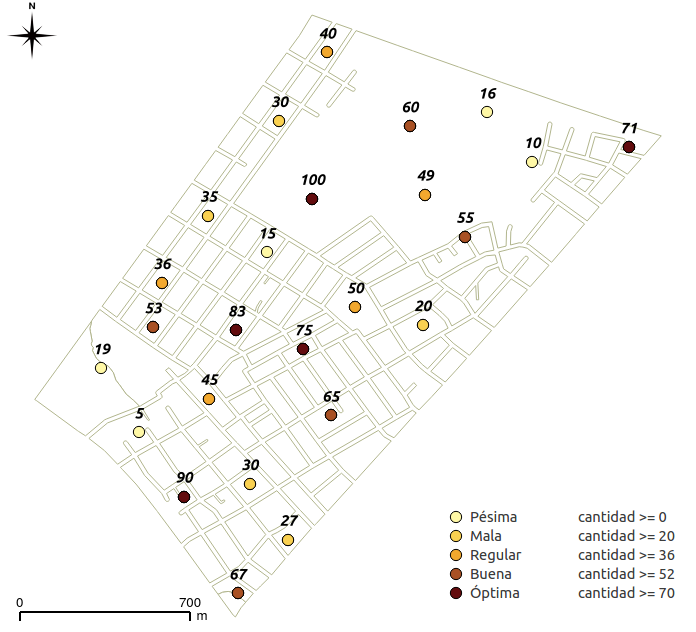
\includegraphics[width=0.9\textwidth]{./capitulo-6/graphics/extension-poblacion.png}
\caption{\label{fig:distribucion-puntos}Distribución geográfica de los 25 puntos de control.}
\end{figure}


\subsection{Periodo y datos climatológicos}
La mayoría de los estudios, que posteriormente fueron utilizados para las comparaciones, se basan
en someter a un grupo de individuos por un periodo de tiempo fijo utilizando una temperatura
constante. El mayor periodo observado fue de $46,83$ días en \cite{rueda1990temperature}, motivo
por el cual el tamaño del periodo fue establecido en 50 días.

En total se realizaron 10 iteraciones de 50 días cada una con las siguientes temperaturas :
15\textcelsius , 18\textcelsius , 20\textcelsius , 22\textcelsius , 24\textcelsius , 25\textcelsius
, 26\textcelsius , 27\textcelsius , 30\textcelsius , 34\textcelsius. De este modo se pueden simular
el proceso evolutivo de los individuos de la población a 10 temperaturas constantes.

\begin{figure}[!htpb]
\centering
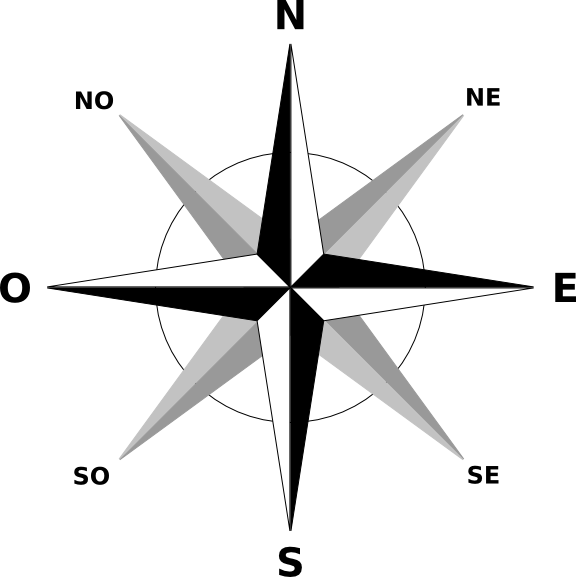
\includegraphics[width=0.5\textwidth]{./capitulo-6/graphics/rosa-de-vientos.png}
\caption{\label{fig:puntos-cardinales}Representación de los puntos cardinales.}
\end{figure}

La dirección al igual que la temperatura fue establecida como una constante para las pruebas, para
facilitar el análisis de la dispersión de los focos. La dirección del viento seleccionada fue la
suroeste (\figref{fig:puntos-cardinales}), que genera un ángulo que varía entre $202,5^{\circ}$ a
$247,5^{\circ}$.

\subsection{Parámetros de simulador del proceso evolutivo}
Los parámetros del simulador del proceso evolutivo, en su mayoría son calculados con datos
biológicos correspondientes al área de estudio. Obtener dichos datos requieren minuciosos estudios
de campo que escapan del alcance de este trabajo. Finalmente se optó por utilizar configuraciones
provenientes del material bibliográfico disponible que utilizado para el diseño y desarrollo del
modelo encargado de realizar la simulación de la ecología del vector.

El tamaño del radio, $r$, fue configurado en $200$ metros, para el cálculo de la densidad relativa
de larvas, $u(x,y)$ (ver \secref{subsec:cap4-zonificacion}). De este modo se incluirán todos los
puntos de control que se encuentren en un área de $125,663 \times 10^{3}$ $m^{2}$.

En cuanto a los sitios de reproducción, los parámetros $bs_{min}$ y $bs_{max}$ fueron tomados
configurados según lo observado en \cite{otero2006stochastic, otero2008stochastic}, siendo $15$ y
$50$ los valores adoptados respectivamente.  El valor de $bs_{med}$ fue establecido, en $32,5$,
realizando un promedio entre $bs_{min}$ y $bs_{max}$.

En la \tabref{tab:coef-sharpe-demichele}, se pueden apreciar los coeficientes para el modelo
simplificado de Sharpe y DeMichele, con inhibición de altas temperaturas de Schoolfield (ver
\secref{subsec:cap4-tasas de desarrollo}) utilizados para calcular las tasas de desarrollo media
en $dias^{-1}$ fueron tomados de : \cite{rueda1990temperature} para el desarrollo larvario y el
desarrollo pupal, y de \cite{otero2006stochastic} para la eclosión de huevos, ciclo gonotrófico para hembras nulíperas y paridas.

\begin{table}[!htpb]
\begin{minipage}{\textwidth}
    \centering
    \caption{ \label{tab:coef-sharpe-demichele} Coeficientes para el modelo simplificado de Sharpe y DeMichele, con inhibición de altas temperaturas presentado por Schoolfield.}
    \begin{tabular}{p{6cm} c r r r r }
        \hline \\
        Ciclo de desarrollo    & $R(298K)$ & $\Delta H_{A}$ & $\Delta H_{H}$ & $\Delta T_{1/2}$  \\
        \hline
        \hline\\
        Eclosión de los huevos$^a$ & 0,24000 & 10798,00 &  100000,00  & 14184,000\\
        Desarrollo larvario$^b$    & 0,20429 & 36072,78 &   59147,51  &   301,560\\
        Desarrollo pupal$^b$       & 0,74423 & 19246,42 &    5954,35  &   302,687\\
        Ciclo gonotrófico (AN)$^c$ & 0,21600 & 15725,00 & 1756481,00  &   447,200\\
        Ciclo gonotrófico (AP)$^c$ & 0,37200 & 15725,00 & 1756481,00  &   447,200\\
    \end{tabular}
    \footnotetext[1]{Coeficientes tomados \cite{otero2006stochastic}.}
    \footnotetext[2]{Coeficientes tomados \cite{rueda1990temperature}.}
    \footnotetext[3]{Coeficientes, para el desarrollo del ciclo gonotrófico de hembras paridas (AP) y nulíparas (AN), tomados \cite{otero2006stochastic}.}
\end{minipage}
\end{table}

Las configuraciones adoptadas de
\cite{otero2006stochastic,otero2008stochastic,rueda1990temperature}, resultan válidas para las
pruebas, sin embargo pueden requerir una revisión general con el fin de realizar los ajustes
correspondientes teniendo en cuenta los datos ecológicos del área de estudio.

\subsection{Hardware y sistema operativo utilizados}
El hardware y el sistema operativo utilizados para realizar las pruebas, tienen las siguientes
características :
\begin{itemize}
\item Procesador : Intel Core i5-2430M
\item CPU : 2.40GHz × 4
\item Memoria : 8 GB
\item Sistema operativo : Ubuntu 13.10 x 64
\end{itemize}


\subsection{Tasa de desarollo}
Verificar las tasas de desarrollo de los individuos de la población de forma a validar
si el incremento de la madurez del individuo es correcta. Se debe contar con el tiempo
promedio de de la duración de cada estado, en días, para compararlos con los promedios
generales.

\begin{itemize}
    \item Temperatura constante
    \item Duración en promedio en cada estado a temperatura constante
    \item Desviación estándar
    \item Calcular el error
\end{itemize}

\section{Ciclo gonotrófico}
Para el análisis de la tasa de desarrollo, en días, del ciclo gonotrófico de las hembras del Aedes
aegypti, se clasificó la población en hembras núliparas y paridas. En la
\tabref{tab:ciclo-gonotrofico-test} se puede observar una media de $5,03$ días para las hembras
nulíparas y  $2,92$ días para las paridas para una temperatura aproximada de $25,11$ \textcelsius.

\begin{table}[!htbp]
    \begin{minipage}{\textwidth}
        \centering
        \caption{ \label{tab:ciclo-gonotrofico-test} Análisis de duración del ciclo gonotrófico
        de la hembra de Aedes aegypti nueve temperaturas constantes  (18-34 \textcelsius).}
        \begin{tabular}{l *{10}{c} }
            \hline \\
            & &  & &  & &  &  &  &  & Media\\
            Población & 18\textcelsius & 20 \textcelsius & 22 \textcelsius & 24 \textcelsius
                      & 25 \textcelsius & 26\textcelsius  & 27 \textcelsius & 30 \textcelsius
                      & 34\textcelsius & General\\

            \hline
            \hline \\
            Nulíparas\footnote{Hembras nulíparas que no han ovipuesto.}
                        & 8,97 & 7,4  & 6,13  & 5,08  & 4,63 & 4,22  & 3,85 & 2,94 & 2,06 & 5,03\\
            Paridas\footnote{Hembras que ya han realizado al menos una ovipostura.}
                        & 5,21 & 4,3  & 3,56  & 2,95  & 2,69 & 2,45  & 2,24 & 1,71 & 1,2 & 2,92\\
            Media \footnote{Promedio general de la duración general del ciclo gonotrófico para las
            hembras}
                        & 7,09 & 5,85 & 4,85  & 4,02  & 3,66 & 3,34  & 3,05 & 2,33 & 1,63 & 3,98\\
        \end{tabular}
    \end{minipage}
\end{table}

Las variaciones en la temperatura influyen en tiempo de digestión de la sangre y el
desarrollo de los ovarios, a medida que la temperatura desciende, la digestión y por ende el ciclo
gonotrófico tomará más tiempo (\figref{fig:ciclo-gonotrofico-temperatura}). En \cite{edman1987host}
se observó que hembras nulíparas de Aedes aegypti poseen un proceso de digestión es más lento en
las hembras paridas y por ende el ciclo gonotrófico de las mismas tiene a ser más largo. Existen
diversos estudios, que han reportado que el patrón diario de alimentación de los mosquitos, varia
de acuerdo a las localidades y subespecies. A continuación se mencionaran algunos estudios
realizados correspondientes a la duración del ciclo gonotrófico, con el fin de realizar una
comparación con los resultados obtenidos mediante el proceso evolutivo.

\begin{figure}[!htbp]
    \centering
    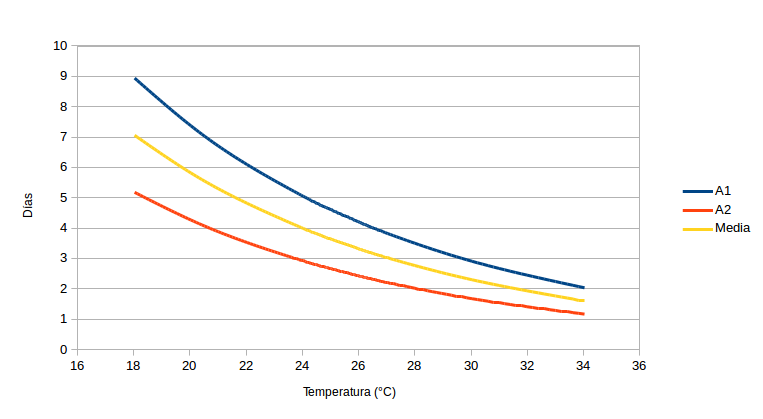
\includegraphics[width=1\textwidth]{capitulo-6/graphics/ciclo-gonotrofico-temperatura.png}
    \caption{\label{fig:ciclo-gonotrofico-temperatura} Tasa de desarrollo, en días, del ciclo
    gonotrófico de hembras nulíparas, hembras paridas y la media general a nueve temperaturas
    constantes (18-34 \textcelsius).}
\end{figure}

En \cite{beltran2001bionomia} se determinó que la duración del ciclo gonotrófico del Aedes
aegypti, para los siguientes municipios de México en, 3 días para Tamazula de Gordiano a una
temperatura de $21,5$ \textcelsius, 3 días para Techaluta de Montenegro a $22,8$ \textcelsius, 4
días para Tuxpan a 22 \textcelsius y 5 días para CD Zacoalco de Torres a $22,7$ \textcelsius.

En \cite{luevano1993ciclo}, el autor determinó la duración del ciclo gonotrófico de las
poblaciones naturales de Aedes aegypti en el área metropolitana de Monterrey, Nuevo León. México,
en cinco días, a una temperatura promedio de $25,5$ \textcelsius.

En \cite{trpis1986dispersal} los autores reportaron una duración del ciclo gonotrófico en Kenia a
nivel rural de, 5 a 7 días para el primer ciclo (hembras nulíparas) y de 4 a 5 días para los
siguientes ciclos (hembras paridas). El método utilizado fue de captura con cebo humano de
mosquitos de Aedes aegypti.

Según \cite{sivanathan2006ecology} el ciclo gonotrófico del aAedes aegypti y Aedes albopictus se
encuentra acotada entre $2,73$ a 3 días respectivamente.

Las diferentes condiciones climáticas y la capacidad de adaptación en habitad específicos, del
Aedes aegypti, son las responsables de diferencias que se puedan tener entre cepas del mosquito.
La duración del ciclo gonotrófico obtenida, depende de los coeficientes para el modelo de
maduración enzimática de \cite{sharpe1977reaction} que fue tomado de \cite{otero2006stochastic},
que según los autores fue tomado de \cite{focks1993dynamic}.


\section{Vuelo y dispersión}
Para el análisis de la distancia recorrida, en metros, del adulto de Aedes aegypti, se realizaron
pruebas a 9 temperaturas constantes (15-34\textcelsius), solo las hembras que han ovipuesto al
menos una vez fueron incluidas. En la tabla \ref{tab:pomedio-vuelo-test} se presentan los
resultados obtenidos para la disperción de las hembras adultas del aedes aegypit agrupadas por el
tipo su tipo de zona, en general se obtuvo un promedio de $65,74$, $63,97$ $1308,19$ metros para las zonas buena, normal y malas respectivamente. Existen diversos estudios, que han reportado que
la disperción del aedes aegypti en relación a las caracteristicas de su ambiente. A continuación
se mencionaran algunos estudios realizados, con el fin de realizar una comparación con los resultados obtenidos.

En \cite{cabezas2005dengue} señalan que por lo general mosquito no sobrepasa los 50 a 100 metros
durante su vida, ya que tiende a permanecer en el lugar donde emergió.

Según \cite{ThironIzcazaJ2003} por lo general, la hembra de Ae. aegypti, permanece físicamente en
donde emergió, siempre y cuando no halla algún factor que la perturbe o no disponga de huéspedes,
sitios de reposo y de postura. En caso de no haber recipientes adecuados, la hembra grávida es capaz de volar hasta tres kilómetros en busca de este sitio.

Los autores de \cite{dengueUruguayCap8} señalan que, para las estrategias de control de Aedes
aegypti en zonas urbanas donde existen brotes de dengue y fiebre amarilla se asume que los
mosquitos tienen un rango de vuelo durante su vida de 50 a 100 metros.

En \cite{luevano1993ciclo} se reporta, que el aedes aegypti es un mosquito doméstico que
generalmente esta confinado a las casas donde se cria, tiene un rango de vuelo corto, entre 23 a 50 metros, y raramente se dispersa a largas distancias.

\cite{mcdonald1977population} en Kenia, liberó poblaciones de Aedes aegypti a las distancias de,
200, 400 y 800 metros, y observó que aproximadamente el 50 \% de los mosquitos marcados se
dispersaron a 200 metros del punto en el cual fueron liberados, un 10 \% a 400 metros y solamente
el 1 \% se dispersó a 800 metros.

En \cite{trpis1986dispersal}, los autores reportaron que en Kenia, que la tasa media de dispersión
de las hembras fue de 57 metros. La distancia máxima de las hembras durante 24 horas fue de 154
metros.

La mayoría de los estudios coinciden que, los adultos del aedes aegypti, en condiciones óptimas de
disponibilidad de alimento y sitios adecuados de ovipostura, tienden a permanecer en el lugar
donde emergieron, con una dispersión media estimada entre 50 y a 100 metros, su presencia es
prácticamente un indicio certero de la proximidad de los criaderos. En caso de no contar con
sitios adecuados de ovipostura y disponibilidad de alimento tienden a dispersarme una mayor
distancia en busca de mejores condiciones.

\begin{table}
    \begin{minipage}{\textwidth}
        \caption{ \label{tab:pomedio-vuelo-test} Análisis de la dispersión, por zona, del adulto
        de Aedes aegypti diez temperaturas constantes (15-34 \textcelsius).}
        \begin{tabular}{p{4cm} *{4}{c}  }
          \hline \\
          Temperatura (\textcelsius)& Buena & Normal & Mala & Media Obtenida\\
          \hline
          \hline \\
          18 & 89,06 & 66,61 & 1274,97 & 476,88\\
          20 & 66,52 & 73,53 & 1516,43 & 552,16\\
          22 & 77,89 & 63,78 & 1003,9 & 381,86\\
          24 & 60,28 & 62,31 & 1077,6 & 400,06\\
          25 & 54,52 & 63,66 & 1397,31 & 505,16\\
          26 & 61,61 & 60,79 & 1509,67 & 544,02\\
          27 & 65,24 & 63,72 & 1433,58 & 520,85\\
          30 & 62,61 & 59,56 & 1213,1 & 445,09\\
          34 & 53,92 & 61,75 & 1347,13 & 487,6\\
          Media General & 65,74 & 63,97 & 1308,19 & 479,3\\
        \end{tabular}
    \end{minipage}
\end{table}

\section{Distribución de Sexo}
Se realizó un análisis para determinar la distribución del sexo del Aedes aegypti. Según
\cite{otero2006stochastic}, alrededor de la mitad de los adultos emergentes son hembras, y se
define una proporción de 1.02:1 macho: hembra. Los autores de \cite{manrique1998desarrollo} la
proporción sexual promedio de adultos emergidos es de $3$ machos por $2,75$ hembras, lo cual no representa una diferencia significativa de una relación 1:1 en las proporciones sexuales.

En general se realizaron pruebas variando la cantidad de individuos de la población, los
resultados se pueden apreciar en la tabla \tabref{tab:distribucion-sexo-test}, donde se observa que
existe una relación 1:1 para la distribución del sexo de los mosquitos.

\begin{table}
    \centering
        \caption{ \label{tab:distribucion-sexo-test} Análisis de la distribución del sexo de Aedes
        aegypti.}
        \begin{tabular}{l c c c }
            \hline \\
            Total de & Adultos & Adultos & Relación \\
            adultos  & machos  & hembras & (macho:hembra) \\
            \hline
            \hline \\
            912    &  461    &  451    &  0,99 : 1,01 \\
            1581   &  812    &  769    &  0,97 : 1,03 \\
            4154   &  2084   &  2070   &  1    : 1 \\
            9722   &  4940   &  4782   &  0,98 : 1,02 \\
            9045   &  4472   &  4573   &  1,01 : 0,99 \\
            16248  &  8104   &  8144   &  1    : 1 \\
            30693  &  15418  &  15275  &  1    : 1 \\
            28411  &  14224  &  14187  &  1    : 1 \\
        \end{tabular}
\end{table}

